\documentclass[11pt, a4paper]{article}

\usepackage[margin=2.2cm]{geometry}
\usepackage[T1]{fontenc}
\usepackage[utf8]{inputenc}
\usepackage{lmodern}
\usepackage{amsmath, amssymb, bm}
\usepackage{booktabs}
\usepackage{xcolor}
\usepackage{hyperref}
\usepackage[round,authoryear,sort]{natbib}
\usepackage{enumitem}
\usepackage{mdframed}
\usepackage{tikz}
\usepackage{titlesec}
\usepackage{float}
\usepackage{parskip}

\usetikzlibrary{positioning, arrows.meta, shapes.geometric}

\hypersetup{colorlinks=true, linkcolor=blue!70!black, urlcolor=blue!70!black, citecolor=blue!70!black}

\definecolor{imperialblue}{RGB}{0,62,116}
\definecolor{lightblue}{RGB}{212,232,245}
\definecolor{lightyellow}{RGB}{255,252,220}
\definecolor{lightgreen}{RGB}{220,245,220}
\definecolor{lightred}{RGB}{255,230,225}
\definecolor{actionblue}{RGB}{225,240,255}

\titleformat{\section}{\large\bfseries\color{imperialblue}}{\thesection.}{0.5em}{}[\vspace{-2pt}\rule{\linewidth}{0.4pt}]
\titleformat{\subsection}{\normalsize\bfseries}{\thesubsection.}{0.5em}{}

\newcommand{\bq}{\bm{q}}
\newcommand{\bp}{\bm{p}}
\newcommand{\bu}{\bm{u}}
\newcommand{\btau}{\bm{\tau}}
\newcommand{\bF}{\bm{F}}
\newcommand{\bM}{\bm{M}}
\newcommand{\bC}{\bm{C}}
\newcommand{\bG}{\bm{G}}
\newcommand{\bJ}{\bm{J}}

\newmdenv[backgroundcolor=lightblue, linecolor=imperialblue!60,
          linewidth=1pt, innerleftmargin=8pt, innerrightmargin=8pt,
          innertopmargin=6pt, innerbottommargin=6pt, skipabove=6pt]{infobox}
\newmdenv[backgroundcolor=lightyellow, linecolor=orange!60,
          linewidth=1pt, innerleftmargin=8pt, innerrightmargin=8pt,
          innertopmargin=6pt, innerbottommargin=6pt, skipabove=6pt]{warnbox}
\newmdenv[backgroundcolor=lightgreen, linecolor=green!50!black,
          linewidth=1pt, innerleftmargin=8pt, innerrightmargin=8pt,
          innertopmargin=6pt, innerbottommargin=6pt, skipabove=6pt]{successbox}
\newmdenv[backgroundcolor=actionblue, linecolor=blue!50,
          linewidth=1pt, innerleftmargin=8pt, innerrightmargin=8pt,
          innertopmargin=6pt, innerbottommargin=6pt, skipabove=6pt]{actionbox}

\title{\textbf{Meeting Notes: Ball-in-Cup Experimental Platform}\\[4pt]
       \large Two-Rail Human Control Task, Disturbance Adaptation, and Sample-Size Planning}
\author{Dipankar Bhattacharya}
\date{26 May 2026}

\begin{document}

\maketitle
\tableofcontents
\vspace{0.5cm}
\hrule
\vspace{0.4cm}

\section{Overview}

This meeting focused on the design of a human experiment built around a ball-in-cup task on a two-axis manual rail platform. The main goals are to study sensorimotor learning, disturbance adaptation, and muscle activity during repeated trials.

\begin{infobox}
\textbf{Overarching aim.} Develop a human-inspired stiffness modulation framework for elbow exosuits that could assist people with Parkinson's disease and related neurological disorders affecting movement stability and coordination. Healthy human demonstrations on the rail platform provide the target impedance behaviour; a cable-driven manipulator with an antagonistic exosuit replicates and learns that behaviour through a three-phase pipeline (Phase~1: human reference, Phase~2: digital twin + RL, Phase~3: real-robot validation via exo-cable stiffness).
\end{infobox}

\begin{infobox}
\textbf{Core idea:} the participant manipulates a two-rail platform by hand, while a ball in a cup provides a coupled stabilization task. Platform motion, force/torque sensing, camera-based ball tracking, and EMG are all used to study learning and adaptation.
\end{infobox}

\section{Experimental Platform Concept}

The proposed setup consists of two stacked linear rails that provide orthogonal motion:

\begin{itemize}[nosep]
  \item the bottom rail moves left and right,
  \item the upper rail moves up and down,
  \item a cup with a ball sits on the top stage,
  \item the participant moves the system using a handle mounted beneath the cup.
\end{itemize}

A 6-axis force/torque sensor will be placed beneath the cup. Its signals will be calibrated against camera-based measurements of the ball position. The long-term goal is to estimate the ball location from force/torque signals, possibly using a regression-based mapping.

Relevant sensor channels are expected to include:

\begin{itemize}[nosep]
  \item $F_x$ and $F_y$,
  \item $M_x$ and $M_y$,
  \item other channels if they improve the regression model.
\end{itemize}

\section{Experimental Blocks}

The block protocol has been moved under the phase-first workflow in
Section~\ref{sec:phasewise-transfer}, specifically under
Phase 1 (human rail experiment). This keeps the narrative in execution order:
Phase 1 (human rail), Phase 2 (exo + manipulator), and Phase 3 (manipulator-only).

\section{Additional Human Measurements}

EMG data will be recorded during the trials. This will allow us to examine muscle activation patterns as participants learn the task and respond to perturbations.

Potential questions include:

\begin{itemize}[nosep]
  \item whether muscle activation changes with practice,
  \item whether adaptation is associated with altered co-contraction,
  \item how EMG patterns change when the disturbance is introduced.
\end{itemize}

\section{Ball Position Estimation and Calibration}

Because the ball position is not directly measured by the force sensor, a calibration procedure is needed. The plan is to use synchronized camera tracking and force/torque recordings to build a mapping from sensor outputs to ball position.

A simple workflow is:

\begin{enumerate}[nosep]
  \item track the true ball position with a camera,
  \item record force/torque data at the same time,
  \item fit a regression model to map sensor signals to ball location,
  \item validate the estimator on held-out data.
\end{enumerate}

Possible estimation models include linear regression, polynomial regression, or a nonlinear machine-learning model if needed.

\section{Sample Size and Participant Number}

We also discussed how to determine the number of participants needed. The plan is to use an a priori power analysis.

The sample size depends on:

\begin{itemize}[nosep]
  \item the primary outcome measure,
  \item the main hypothesis or comparison,
  \item the expected effect size,
  \item the chosen significance level and power.
\end{itemize}

A common starting point is $\alpha = 0.05$ and power $= 0.80$. The participant number can then be estimated once the main behavioral variable is chosen. Candidate primary outcomes include ball-position error, time inside the target circle, number of boundary violations, recovery time after disturbance, or a main EMG metric.

For a within-subject comparison, such as early versus late disturbance trials, a paired-difference analysis can use
\texttt{TTestPower} in \texttt{statsmodels}.
A simple approximation is

\begin{equation}
  n \approx \left( \frac{z_{1-\alpha/2} + z_{1-\beta}}{d_z} \right)^2,
\end{equation}

where $d_z$ is the standardized effect size for the paired difference, $\alpha$ is the false-positive rate, and $1-\beta$ is the desired power.

\textbf{Example:} if pilot data suggest that the disturbance increases ball-position error by $\Delta = 4$ units, and the standard deviation of the paired differences is $\sigma_d = 6$ units, then $d_z = \Delta / \sigma_d = 0.67$. Using \texttt{statsmodels} with $\alpha = 0.05$ and power $= 0.80$ gives

\begin{equation}
  n \approx 19.5.
\end{equation}

So the study would need about 20 participants for the minimum estimate, and it would be prudent to recruit a few extra participants to account for unusable trials or dropouts.

The preferred approach is to use a previous similar paper or pilot data to estimate the expected effect size, then compute the required sample size in Python using \texttt{statsmodels}. For example, in Python one could write:

\begin{verbatim}
from statsmodels.stats.power import TTestPower
power_analysis = TTestPower()
nobs = power_analysis.solve_power(effect_size=0.67,
                                  alpha=0.05,
                                  power=0.80,
                                  alternative='two-sided')
\end{verbatim}

\begin{warnbox}
If prior literature is too weak to support a reliable effect-size estimate, a small pilot study should be run first.
\end{warnbox}

\subsection{Participant Numbers Reported in Similar Studies}

To anchor our estimate in published practice, the table below summarises participant counts and effect-size hints from comparable cup--ball and complex-object manipulation studies. The local paper folder already contains the first three entries; the others are drawn from related online literature.

\begin{center}
{\small
\begin{tabular}{p{0.34\linewidth}p{0.10\linewidth}p{0.48\linewidth}}
\toprule
\textbf{Study} & \textbf{$N$} & \textbf{Notes on design and effect size} \\
\midrule
\citet{bazzi2018} & 10 & Cart--pendulum cup proxy; contraction analysis; large within-subject differences between assistive and resistive perturbation conditions. \\
\citet{razavian2021} & 4 & Pilot-style comparison of four motor-control models. \\
\citet{razavian2023} & 11 & $2\times 2$ design (object type $\times$ perturbation), 4 blocks of 100 trials per participant. \\
\citet{bazzi2020} & 10 & CCM-based robustness analysis with practice. \\
\citet{nayeem2021} & 10--12 & Preparatory movement and initial conditions for complex object transport. \\
\citet{hasson2012} & 14 & Within-subject manipulation of cup--ball; reported large within-subject practice effects, $d_z \approx 0.7$--$1.0$. \\
\citet{lokesh2024} & 12 & Underactuated object control; within-subject adaptation effects $d_z \gtrsim 0.6$. \\
\citet{casadio2006} & 12 & Healthy participants on impedance-modulated robotic platform. \\
\citet{ajoudani2012icra} & 8 & Stiffness transfer from human EMG to manipulator. \\
\bottomrule
\end{tabular}}
\end{center}

\textbf{What this means for our study.} Most cup--ball / complex-object manipulation papers in this line of work use roughly $N=10$--$15$ healthy participants for within-subject designs, and report standardised effect sizes for practice or perturbation effects of approximately $d_z \approx 0.6$--$1.0$. Plugging these into the power formula gives:

\begin{itemize}[nosep]
  \item $d_z = 0.5$ (small--medium): $n \approx 34$,
  \item $d_z = 0.67$ (our working example): $n \approx 20$,
  \item $d_z = 0.8$ (medium--large): $n \approx 15$,
  \item $d_z = 1.0$ (large, typical of Sternad-lab within-subject practice effects): $n \approx 10$.
\end{itemize}

A reasonable target range for our protocol is therefore $N \approx 12$--$20$ healthy participants, depending on the chosen primary outcome. We would aim for the higher end if the primary outcome is EMG-based (more variable across participants) and the lower end if it is a within-subject kinematic measure with strong practice effects.

\section{How the Pieces Connect}

We clarified the intended long-term pipeline for the manipulator and exosuit. The human experiments are performed with healthy participants, and their hand motion provides the reference behavior. The robot side then uses a weak or compliant manipulator, with exo joint stiffness mounted on the manipulator, to mimic an ``unhealthy'' or impaired hand-like interaction.

The connection is easiest to think about in stages:

\begin{itemize}[nosep]
  \item The healthy human initially performs the task and provides the reference behavior.
  \item EMG, rail motion, force/torque, and ball-position data are recorded together.
  \item On the robot side, the exo is mounted on the manipulator and used to change the joint stiffness.
  \item The weak or compliant manipulator then mimics the reduced control capacity of an impaired hand.
  \item A policy is learned from the recorded data, possibly using RL or imitation learning methods.
  \item That learned policy is then transferred to the manipulator, so the manipulator stiffness and response match the desired interaction behavior.
\end{itemize}

In this sense, the exo is not the final goal by itself. It acts as an intermediate teaching and stabilization mechanism on the manipulator. It changes the closed-loop dynamics, provides a richer data set, and helps define what a good control strategy looks like before the manipulator is asked to do the same job autonomously.

This also explains the phrase ``the manipulator will learn from the exo.'' What we mean is that the exo mounted on the manipulator generates a stiffness profile and interaction pattern that can later be distilled into the manipulator controller. The manipulator then becomes the system that executes the learned behavior, while the healthy human data serve as the reference and the exo-on-manipulator trials provide the robot-side adaptation signal.

One practical way to frame the project is:

\begin{enumerate}[nosep]
  \item healthy hand control defines the target behavior,
  \item exo-mounted manipulator trials collect the robot-side training data,
  \item RL or imitation learning learns the policy,
  \item the manipulator implements the policy on the rail platform,
  \item adaptation is evaluated by comparing performance before and after the exo-informed training.
\end{enumerate}

So the connection is: healthy human behavior provides the template, the exo on the manipulator shapes the stiffness and interaction response, and the manipulator eventually inherits the learned control policy.

Two examples make this clearer.

\begin{itemize}[nosep]
  \item \textbf{Example 1: smooth tracking.} A healthy participant moves the rail to the right, the ball begins to drift, and the hand makes a small corrective motion to keep the ball near the target. On the robot side, the manipulator is given a weak or compliant joint stiffness, and the exo mounted on the manipulator adjusts that stiffness so the same correction pattern becomes measurable and repeatable. The exo-on-manipulator trial records the resulting response together with EMG and force data. Later, the manipulator is trained to reproduce the same rightward motion plus correction, so it behaves like the healthy hand template.
  \item \textbf{Example 2: disturbance recovery.} A solenoid push perturbs the rail toward the participant. The healthy participant reacts by changing hand force and timing to bring the ball back into the target region. On the robot side, the manipulator starts from a weak stiffness setting, and the exo mounted on the manipulator modulates stiffness to recover the task. RL can use this repeated disturbance-response data to learn a policy that rewards recovery speed and low ball error. The manipulator then uses that learned policy to generate the same compensatory response without the human hand.
\end{itemize}

In both cases, we are not just copying a path in space. We are trying to copy the interaction rule: how a healthy hand reacts to error, how the robot stiffness changes the response, how quickly it corrects, and how it adapts when the exo or disturbance changes the dynamics.

Another useful way to say it is that the exo mounted on the manipulator can serve as a \emph{teacher} of interaction dynamics. It can make the task easier, more repeatable, or more measurable, which improves the data used for learning. The manipulator is the \emph{student} that later executes the learned stiffness and control behavior on the rail platform.

\begin{figure}[H]
\centering
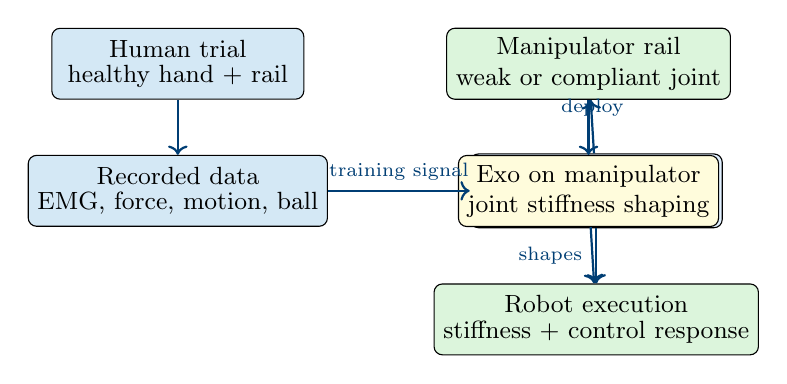
\begin{tikzpicture}[node distance=0.7cm and 1.25cm,
  box/.style={draw, rounded corners=3pt, minimum width=3.2cm, minimum height=0.9cm, align=center, font=\small},
  humanbox/.style={box, fill=lightblue},
  robotbox/.style={box, fill=lightgreen},
  exobox/.style={box, fill=lightyellow},
  arr/.style={->, thick, color=imperialblue}]
  \node[humanbox] (human) {\shortstack{Human trial\\healthy hand + rail}};
  \node[humanbox, below=of human] (human2) {\shortstack{Recorded data\\EMG, force, motion, ball}};
  \node[box, right=1.8cm of human2, fill=actionblue] (policy) {\shortstack{Learned policy\\RL / imitation}};
  \node[robotbox, right=1.8cm of human] (manip) {\shortstack{Manipulator rail\\weak or compliant joint}};
  \node[exobox, below=of manip] (exo) {\shortstack{Exo on manipulator\\joint stiffness shaping}};
  \node[robotbox, below=of policy] (robotout) {\shortstack{Robot execution\\stiffness + control response}};

  \draw[arr] (human) -- (human2);
  \draw[arr] (human2) -- node[above,font=\scriptsize]{training signal} (policy);
  \draw[arr] (policy) -- node[above,font=\scriptsize]{deploy} (manip);
  \draw[arr] (manip) -- (exo);
  \draw[arr] (exo) -- node[left,font=\scriptsize]{shapes} (robotout);
  \draw[arr] (policy) -- (robotout);
\end{tikzpicture}
\caption{Final experiment diagram. Healthy human rail trials provide the template, and the learned policy is transferred to the manipulator rail with exo-shaped stiffness.}
\label{fig:final-system}
\end{figure}

\section{Relevant Literature and Design Implications}

The closest line of work from Dagmar Sternad's group is on humans controlling dynamically complex objects, such as cup--pendulum or cup--ball systems. The main message is that humans do not simply move the object along a geometric path. They exploit stability, predictability, impedance, and task dynamics.

\begin{center}
{\small
\begin{tabular}{p{0.28\linewidth}p{0.34\linewidth}p{0.28\linewidth}}
\toprule
\textbf{Relevant work} & \textbf{Main idea} & \textbf{Implication for our experiment} \\
\midrule
\citet{bazzi2020}; \citet{bazzi2018} & Humans route trajectories through stable or contracting regions when manipulating complex objects. & Analyze whether healthy participants learn rail motions that make the ball dynamics more predictable and robust. \\
\citet{razavian2021}; \citet{razavian2023} & Mechanical impedance and body mechanics strongly shape interaction behavior; fast recovery can arise before neural feedback is available. & Treat exo stiffness on the manipulator as an artificial body-mechanics layer, not just an actuator. \\
\citet{nayeem2021} & Initial conditions and preparatory movements can simplify interaction with complex objects. & Include a preparatory phase before the rail movement; measure whether participants set up the cup/ball state before moving. \\
\citet{lokesh2024}; \citet{lokesh2025} & Humans adapt to uncertain underactuated object dynamics by improving stability and impedance. & Use uncertainty in ball position or rail disturbance as a controlled difficulty variable. \\
\citet{nayeem2022} & Functional object interactions can be quantified after stroke. & The weak manipulator can emulate impaired interaction safely before testing patient populations. \\
\bottomrule
\end{tabular}}
\end{center}

This literature suggests that our outcome measures should not be limited to final task success. We should also measure how participants shape interaction dynamics:

\begin{itemize}[nosep]
  \item whether ball trajectories become more predictable over trials,
  \item whether the rail motion enters more stable regions before perturbations,
  \item whether force/torque signals become smoother or lower variance,
  \item whether EMG shows reduced co-contraction or better timed activation,
  \item whether exo-shaped manipulator stiffness reproduces the healthy interaction pattern.
\end{itemize}

\subsection{Online Literature on Impairment Emulation, Impedance Transfer, and RL Stiffness Policies}

To ground our specific approach in the wider research community, we surveyed online literature addressing: (i)~robotic emulation of paretic or impaired motor capabilities, (ii)~imitation-based stiffness or impedance transfer from human/exo to mechanical manipulators, and (iii)~reinforcement learning for variable impedance controllers.

\begin{enumerate}
  \item \textbf{Emulating Motor Impairment on Robotic Testbeds:}
  In rehabilitation engineering, researchers routinely configure robotic manipulators or haptic interfaces with low gains or active compliant modes to emulate paretic, spastic, or neurologically weak human limbs. For instance, \citet{casadio2006} and \citet{patinvoh2020} have programmed robots to mimic the asymmetric force field, muscle weakness, or tremor characteristic of a post-stroke upper limb. This supports our strategy of using a weak or highly compliant joint stiffness setting on the manipulator to mimic the ``unhealthy'' baseline interaction.

  \item \textbf{Human-to-Robot Impedance and Stiffness Transfer:}
  A well-established paradigm in physical human-robot interaction is the extraction of biological impedance profiles to teach robotic systems how to handle unstable tasks. Seminal work by \citet{ajoudani2012icra} and \citet{ajoudani2018springer} on the ``Tele-impedance'' framework demonstrated how human hand stiffness can be estimated online via multi-channel EMG and transferred in real-time to a robot manipulator. Furthermore, \citet{kronander2014} and \citet{rozo2015} developed methods for a robot to learn variable impedance behaviors directly from active human demonstration and physical human-robot interaction (pHRI). In our project, rather than active human guidance, the exo acts as the hardware mediator that physically enforces the targeted impedance profile on the weak manipulator. The manipulator then ``learns from the exo'' by digesting these physically assisted interaction trials into a parametric impedance controller.

  \item \textbf{Reinforcement Learning for Variable Impedance Control (VIC-RL):}
  Our proposed policy learning step (using RL to discover optimal stiffness behaviors) matches the Variable Impedance Control via Reinforcement Learning line of research pioneered by \citet{buchli2011} and extended by \citet{bogdanovic2020}. In these papers, the RL action space represents virtual joint or Cartesian stiffness matrix parameters ($K, B$) instead of raw torques or position targets. This approach is highly robust and matches our proposed controller design because:
  \begin{itemize}[nosep]
    \item it guarantees passivity and safety during learning (since the robot behaves as a passive spring-damper system relative to the rail),
    \item it naturally accommodates the low or high stiffness regimes that the exo generates, and
    \item it avoids high-frequency corrective torques, leading to smooth, hand-like interactions.
  \end{itemize}
\end{enumerate}

\subsection{Alternative Experimental Framing}

There are at least three useful ways to frame the experiment.

\begin{enumerate}[nosep]
  \item \textbf{Human motor-learning experiment:} healthy participants learn the rail--cup--ball task, and we study how stability, predictability, and EMG change with practice.
  \item \textbf{Robot emulation experiment:} the weak manipulator tries to reproduce healthy hand interaction, while the exo mounted on the manipulator adjusts joint stiffness.
  \item \textbf{Rehabilitation-inspired transfer experiment:} healthy behavior defines the target, the weak manipulator represents impaired control, and the exo stiffness becomes the teaching signal that the manipulator learns from.
\end{enumerate}

These framings are compatible. The first provides the human reference, the second builds the robot imitation, and the third connects the work to rehabilitation.

\section{Linear Rail Experiment Setup Requirements}

A good rail setup should be simple enough for ethics approval and repeatable enough for modeling. The safest initial design is a manually actuated two-axis table-top rail with software and mechanical limits, before adding the manipulator-driven version.

\begin{center}
{\small
\begin{tabular}{p{0.25\linewidth}p{0.62\linewidth}}
\toprule
\textbf{Subsystem} & \textbf{Recommended requirement} \\
\midrule
Rails & Two orthogonal low-friction linear rails with hard mechanical end stops; travel should be large enough for the task but short enough to prevent excessive reach. \\
Handle & Comfortable handle below the cup, rounded edges, no pinch points, and adjustable height for participant posture. \\
Cup and ball & Transparent or camera-visible cup, replaceable balls with known mass/radius, and removable target marker inside the cup. \\
Sensing & 6-axis force/torque sensor under the cup, rail encoders or linear scales, overhead camera for calibration, and synchronized EMG. \\
Disturbance & Solenoid or voice-coil actuator with adjustable amplitude, short pulse duration, physical stroke limit, and software lockout. \\
Safety & Emergency stop, software travel limits, mechanical stops, current limits, guarded pinch zones, and operator-controlled trial start. \\
Data & Common timestamp for EMG, force/torque, rail position, camera, auditory feedback, and disturbance trigger. \\
\bottomrule
\end{tabular}}
\end{center}

\begin{figure}[H]
\centering
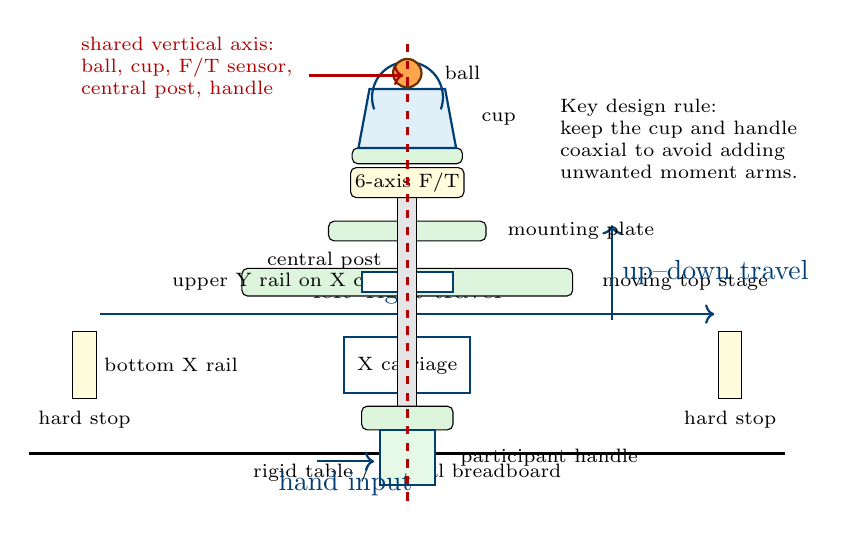
\begin{tikzpicture}[x=1cm,y=1cm,
  part/.style={draw, rounded corners=2pt, fill=lightblue, align=center, font=\small},
  plate/.style={draw, rounded corners=2pt, fill=lightgreen, align=center, font=\small},
  sensor/.style={draw, rounded corners=2pt, fill=lightyellow, align=center, font=\scriptsize},
  note/.style={align=center, font=\scriptsize},
  arr/.style={->, thick, color=imperialblue}]
  \draw[very thick] (-4.8,-1.55) -- (4.8,-1.55);
  \node[note, below] at (0,-1.55) {rigid table / optical breadboard};

  \draw[part, minimum width=7.6cm, minimum height=0.35cm] (0,-0.85) rectangle (0,0);
  \node[note] at (-3.0,-0.42) {bottom X rail};
  \draw[fill=white, draw=imperialblue, thick] (-0.8,-0.78) rectangle (0.8,-0.07);
  \node[note] at (0,-0.43) {X carriage};
  \draw[arr] (-3.9,0.22) -- (3.9,0.22) node[midway, above] {left--right travel};
  \draw[fill=lightyellow, draw] (-4.25,-0.85) rectangle (-3.95,0);
  \draw[fill=lightyellow, draw] (3.95,-0.85) rectangle (4.25,0);
  \node[note] at (-4.1,-1.12) {hard stop};
  \node[note] at (4.1,-1.12) {hard stop};

  \draw[plate, minimum width=4.2cm, minimum height=0.35cm] (-2.1,0.45) rectangle (2.1,0.8);
  \node[note] at (-1.35,0.63) {upper Y rail on X carriage};
  \draw[fill=white, draw=imperialblue, thick] (-0.58,0.5) rectangle (0.58,0.75);
  \node[note, right] at (2.35,0.63) {moving top stage};
  \draw[arr] (2.6,0.15) -- (2.6,1.35) node[midway, right] {up--down travel};

  \draw[plate, minimum width=2.0cm, minimum height=0.25cm] (-1.0,1.15) rectangle (1.0,1.4);
  \node[note, right] at (1.15,1.28) {mounting plate};
  \draw[fill=gray!20, draw] (-0.12,-1.25) rectangle (0.12,1.95);
  \node[note, left] at (-0.2,0.9) {central post};

  \draw[sensor, minimum width=1.45cm, minimum height=0.38cm] (-0.72,1.7) rectangle (0.72,2.08);
  \node[note] at (0,1.89) {6-axis F/T};
  \draw[plate, minimum width=1.4cm, minimum height=0.2cm] (-0.7,2.13) rectangle (0.7,2.33);
  \draw[draw=imperialblue, thick, fill=lightblue!70] (-0.62,2.33) -- (0.62,2.33) -- (0.48,3.08) -- (-0.48,3.08) -- cycle;
  \draw[draw=imperialblue, thick] (-0.42,2.82) arc[start angle=200,end angle=-20,radius=0.45cm];
  \node[note, right] at (0.82,2.7) {cup};
  \draw[fill=orange!70, draw=orange!40!black, thick] (0,3.28) circle (0.18);
  \node[note, right] at (0.35,3.28) {ball};

  \draw[plate, minimum width=1.15cm, minimum height=0.3cm] (-0.58,-1.25) rectangle (0.58,-0.95);
  \draw[draw=imperialblue, thick, fill=lightgreen!70] (-0.35,-1.95) rectangle (0.35,-1.25);
  \node[note, right] at (0.55,-1.6) {participant handle};
  \draw[arr] (-1.15,-1.65) -- (-0.42,-1.65) node[midway, below] {hand input};

  \draw[dashed, very thick, red!70!black] (0,-2.15) -- (0,3.65);
  \node[note, text=red!70!black, align=left] at (-2.8,3.35) {shared vertical axis:\\ball, cup, F/T sensor,\\central post, handle};
  \draw[arr, red!70!black] (-1.25,3.25) -- (-0.05,3.25);

  \node[note, align=left] at (3.45,2.45) {Key design rule:\\keep the cup and handle\\coaxial to avoid adding\\unwanted moment arms.};
\end{tikzpicture}
\caption{Physical schematic of the two-rail system. The ball, cup, force/torque sensor, central post, and participant handle are mounted on the same vertical axis so that hand input acts directly beneath the cup.}
\label{fig:rail-setup}
\end{figure}

\begin{figure}[H]
\centering
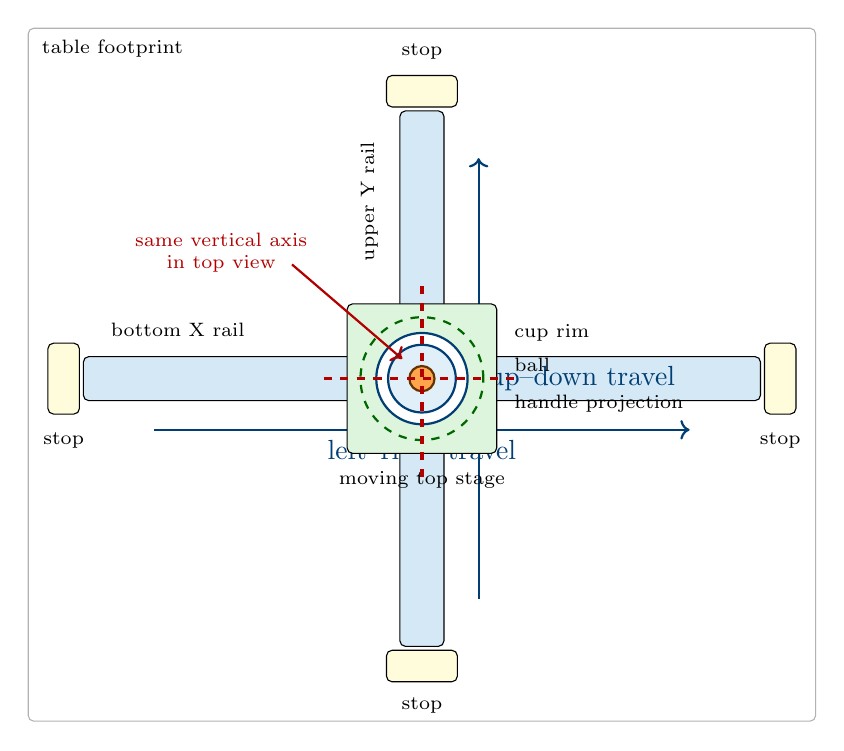
\begin{tikzpicture}[x=1cm,y=1cm,
  rail/.style={draw, rounded corners=2pt, fill=lightblue, align=center, font=\small},
  stage/.style={draw, rounded corners=2pt, fill=lightgreen, align=center, font=\small},
  stop/.style={draw, rounded corners=2pt, fill=lightyellow, align=center, font=\scriptsize},
  note/.style={align=center, font=\scriptsize},
  arr/.style={->, thick, color=imperialblue}]
  \draw[rail] (-4.3,-0.28) rectangle (4.3,0.28);
  \node[note] at (-3.1,0.62) {bottom X rail};
  \draw[arr] (-3.4,-0.65) -- (3.4,-0.65) node[midway, below] {left--right travel};
  \draw[stop] (-4.75,-0.45) rectangle (-4.35,0.45);
  \draw[stop] (4.35,-0.45) rectangle (4.75,0.45);
  \node[note] at (-4.55,-0.78) {stop};
  \node[note] at (4.55,-0.78) {stop};

  \draw[rail] (-0.28,-3.4) rectangle (0.28,3.4);
  \node[note, rotate=90] at (-0.67,2.25) {upper Y rail};
  \draw[arr] (0.72,-2.8) -- (0.72,2.8) node[midway, right] {up--down travel};
  \draw[stop] (-0.45,-3.85) rectangle (0.45,-3.45);
  \draw[stop] (-0.45,3.45) rectangle (0.45,3.85);
  \node[note] at (0,-4.15) {stop};
  \node[note] at (0,4.15) {stop};

  \draw[stage, minimum width=1.9cm, minimum height=1.9cm] (-0.95,-0.95) rectangle (0.95,0.95);
  \node[note] at (0,-1.28) {moving top stage};
  \draw[draw=imperialblue, thick, fill=white] (0,0) circle (0.58);
  \draw[draw=imperialblue, thick, fill=lightblue!70] (0,0) circle (0.43);
  \draw[fill=orange!70, draw=orange!40!black, thick] (0,0) circle (0.16);
  \draw[draw=green!40!black, thick, dashed] (0,0) circle (0.78);
  \node[note, right] at (1.05,0.58) {cup rim};
  \node[note, right] at (1.05,0.18) {ball};
  \node[note, right] at (1.05,-0.32) {handle projection};

  \draw[dashed, very thick, red!70!black] (-1.25,0) -- (1.25,0);
  \draw[dashed, very thick, red!70!black] (0,-1.25) -- (0,1.25);
  \node[note, text=red!70!black] at (-2.55,1.6) {same vertical axis\\in top view};
  \draw[arr, red!70!black] (-1.65,1.45) -- (-0.25,0.25);

  \draw[draw=gray!60, rounded corners=2pt] (-5.0,-4.35) rectangle (5.0,4.45);
  \node[note, below right] at (-4.95,4.43) {table footprint};
\end{tikzpicture}
\caption{Top view of the two-rail system. The X and Y rail axes cross at the top-stage center, where the ball, cup, force/torque sensor, central post, and handle project to the same point.}
\label{fig:rail-top-view}
\end{figure}

\section{Ethics and Safety Protocols}

For ethics approval, the human rail experiment should be described as a low-risk manual interaction task with controlled perturbations. The key point is that the participant is not strapped to an actuator and can release the handle at any time.

Recommended safety measures:

\begin{itemize}[nosep]
  \item Obtain informed consent and explain the disturbance timing, task goals, and right to stop.
  \item Screen participants for recent upper-limb injury, pain, neurological disorder, severe musculoskeletal limitation, or skin sensitivity to EMG electrodes.
  \item Use a familiarization block before the ball and before any disturbance.
  \item Keep the handle passive in the first human experiment; do not rigidly attach the hand or arm.
  \item Add mechanical end stops and software travel limits on both rail axes.
  \item Guard all pinch points around rails, pulleys, solenoids, and moving stages.
  \item Limit disturbance amplitude, duration, and frequency; begin with very small pulses and increase only after pilot safety checks.
  \item Include an emergency stop accessible to the participant and another to the experimenter.
  \item Use trial-by-trial verbal check-ins for fatigue, discomfort, dizziness, or pain.
  \item Stop immediately if the participant reports pain, loses grip, or if sensor readings exceed preset limits.
\end{itemize}

\begin{figure}[H]
\centering
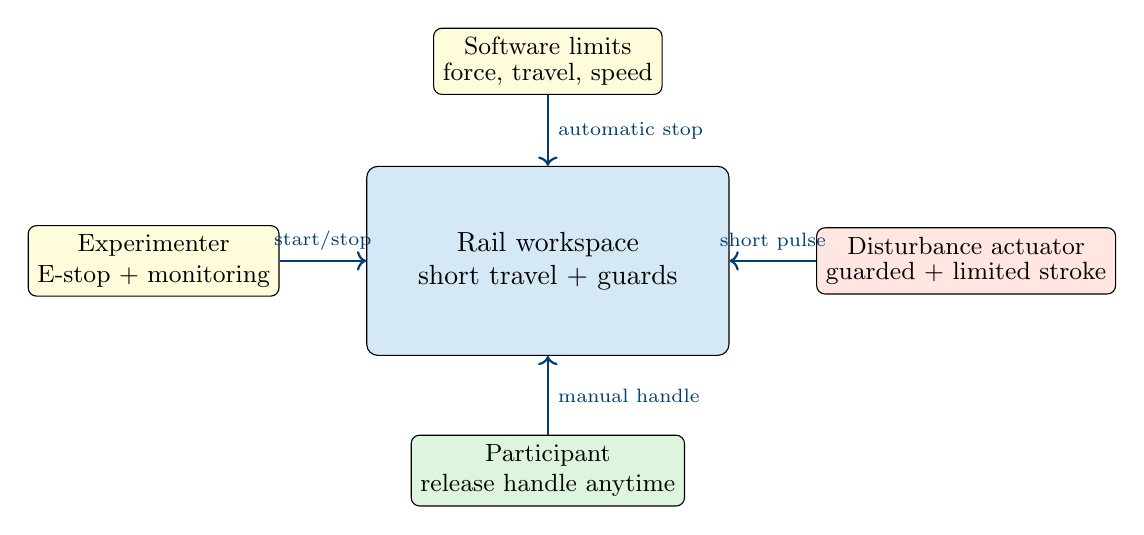
\begin{tikzpicture}[node distance=0.8cm and 1.0cm,
  zone/.style={draw, rounded corners=4pt, minimum width=4.6cm, minimum height=2.4cm, fill=lightblue, align=center},
  box/.style={draw, rounded corners=3pt, minimum width=2.8cm, minimum height=0.75cm, fill=lightgreen, align=center, font=\small},
  safe/.style={draw, rounded corners=3pt, minimum width=2.7cm, minimum height=0.75cm, fill=lightyellow, align=center, font=\small},
  danger/.style={draw, rounded corners=3pt, minimum width=2.7cm, minimum height=0.75cm, fill=lightred, align=center, font=\small},
  arr/.style={->, thick, color=imperialblue}]
  \node[zone] (workspace) {\shortstack{Rail workspace\\short travel + guards}};
  \node[box, below=1.0cm of workspace] (participant) {\shortstack{Participant\\release handle anytime}};
  \node[safe, left=1.1cm of workspace] (op) {\shortstack{Experimenter\\E-stop + monitoring}};
  \node[danger, right=1.1cm of workspace] (actuator) {\shortstack{Disturbance actuator\\guarded + limited stroke}};
  \node[safe, above=0.9cm of workspace] (limits) {\shortstack{Software limits\\force, travel, speed}};
  \draw[arr] (participant) -- node[right,font=\scriptsize]{manual handle} (workspace);
  \draw[arr] (op) -- node[above,font=\scriptsize]{start/stop} (workspace);
  \draw[arr] (actuator) -- node[above,font=\scriptsize]{short pulse} (workspace);
  \draw[arr] (limits) -- node[right,font=\scriptsize]{automatic stop} (workspace);
\end{tikzpicture}
\caption{Top-down ethics and safety schematic. The participant interacts through a releasable handle; the actuator is guarded and limited; the experimenter and software both have stop authority.}
\label{fig:ethics-safety}
\end{figure}

\section{Methodology Adopted from Tele-Impedance (Ajoudani et al., 2012)}
\label{sec:teleimpedance-method}

\citet{ajoudani2012icra} introduced \emph{Tele-Impedance}: a teleoperation
scheme in which a slave robot is commanded with \emph{both} a Cartesian
position reference \emph{and} a stiffness reference estimated in real time
from the agonist--antagonist EMG activity of the human operator.  The
architectural backbone is a \textbf{master--slave pair}: the human operator
performs a task on the master side while the robot simultaneously performs
the same task on the slave side, with human kinematics and impedance
transferred across in real time.

Our experiment uses exactly this architecture:
\begin{itemize}[nosep]
  \item \textbf{Master side --- the two-rail platform.}
        The human participant performs the ball-in-cup task on the physical
        rail rig (Figs.~\ref{fig:rail-setup}--\ref{fig:rail-top-view}).
        The participant wears 8-channel surface EMG on the arm that holds
        the cup handle; a 6-DOF F/T sensor and Optitrack capture handle
        forces and cup position.
  \item \textbf{Slave side --- the SEA cup manipulator with exo-suit.}
        The 2-DOF cable-driven manipulator reproduces the cup trajectory
        commanded from the rail side.  The agonist--antagonist exo cables
        simultaneously receive a co-contraction setpoint derived from the
        participant's EMG, physically realising the impedance modulation
        that matches what the human arm is doing on the rail.
\end{itemize}

This directly mirrors the Ajoudani setup: their human operator caught a ball
on the master side; their KUKA LWR caught the same ball on the slave side,
receiving position \emph{and} stiffness from the operator's EMG. We swap
the KUKA's active Cartesian impedance controller for the SEA exo-cable
co-contraction mechanism, and we swap the free-space ball-catching task for
the constrained rail ball-in-cup task.

\subsection{Master--Slave Architecture}

\begin{center}
\begin{tabular}{p{0.44\linewidth}p{0.50\linewidth}}
\toprule
\textbf{Tele-Impedance --- master / slave} & \textbf{Our system --- rail / manipulator}\\
\midrule
\textit{Master:} human operator performs ball-catch
  & \textit{Master:} participant does ball-in-cup on the 2-rail platform \\
8-channel arm EMG on operator
  & Same 8-channel arm EMG on participant (same muscles, Table~I of paper) \\
Optitrack on wrist / elbow / shoulder
  & Optitrack on cup handle + cart encoder on rail \\
Position signal: operator wrist \(\boldsymbol{\xi}_{human}\)
  & Position signal: cup handle position on rail \((x_{cart},\,y_{cart})\) \\
\textit{Slave:} KUKA LWR executes same ball-catch
  & \textit{Slave:} SEA cup manipulator with exo cables executes same ball-in-cup \\
Slave stiffness command \(\mathbf{K}_{end}\) via KUKA active impedance ctrl
  & Slave stiffness via exo cable co-contraction setpoint
    \(c_{\text{exo}}\in[0,1]\) (dual-groove pulley, SEA springs) \\
6-DOF F/T at slave end-effector
  & 6-DOF F/T at manipulator cup handle; also at rail handle (calibration) \\
Slave position loop: FR Interface, incremental position
  & Slave position loop: computed-torque controller on
    \([q_1,q_2,\dot q_1,\dot q_2]\) (\texttt{controller/computed\_torque\_isaacsim.py}) \\
\bottomrule
\end{tabular}
\end{center}

\textbf{Data flow during a live trial.}
At every control cycle ($\sim$200\,Hz):
\begin{enumerate}[nosep]
  \item Rail Optitrack/encoder sends cup position \((x_c,y_c)\) to the
        manipulator position controller.
  \item 8-channel EMG from the participant's arm is preprocessed to
        envelope \(\mathbf P\).
  \item Null-space projector gives co-contraction signal
        \(\mathbf P_{\text{null}} = (\mathbf I - \hat{\mathbf T}^+
        \hat{\mathbf T})\,\mathbf P\).
  \item Stiffness increment
        \(\Delta\mathbf K = \hat{\boldsymbol\Psi}\,\mathbf P_{\text{null}}\)
        is converted to an exo co-contraction setpoint via the pulley geometry.
  \item Manipulator executes: position from step~1, stiffness from step~4,
        on top of the SEA torque-mode inner loop.
\end{enumerate}
This preserves the two-channel separation of
\citet{ajoudani2012icra}: position and stiffness are transferred through
independent channels, so errors in impedance estimation do not destabilise
the position loop.

\subsection{Two-Stage Offline Calibration}

Calibration is done \emph{on the rail side} (participant at the rail handle,
same posture as Block~B/C), before the main experiment.

\paragraph{Stage 1 --- EMG \(\to\) endpoint-force map \(\hat{\mathbf T}\).}
The rail cart is locked; the participant produces isometric forces of
\(\{5,10,20\}\,\text{N}\) along \(\pm x,\pm y\) while the rail-handle F/T
sensor records ground-truth force.  EMG and force are both recorded;
least-squares regression solves
\[
  \hat{\mathbf T} = \arg\min_{\mathbf T}
  \sum_j \|\mathbf F^{(j)} - \mathbf T\,\mathbf P^{(j)}\|^2.
\]
Protocol: \(4\text{ rep}\times 4\text{ dir}\times 3\text{ level} = 48\)
trials, 60\,s each (first 10\,s discarded).  Target validation:
\(R^2\!\gtrsim\!0.7\) per direction.

\paragraph{Stage 2 --- Null-space EMG \(\to\) stiffness map \(\hat{\boldsymbol\Psi}\).}
Using \(\hat{\mathbf T}\), the null-space projector
\(\mathbf N = \mathbf I - \hat{\mathbf T}^+\hat{\mathbf T}\)
isolates the co-contraction signal \(\mathbf P_{\text{null}}\).
The rail cart now applies \emph{stochastic step perturbations}
(10--20\,mm, 200\,ms duration, random \(xy\) direction) to the participant's
handle at four TCI levels (min, low, med, high).  Endpoint stiffness
\(\mathbf K\) is identified from the perturbation response by fitting a
second-order impedance model
\[
  \mathbf M\ddot{\mathbf X}+\mathbf B\dot{\mathbf X}
  +\mathbf K(\mathbf X-\mathbf X_{eq}) = -\mathbf F
\]
in the frequency domain (0--10\,Hz; \(\mathbf M\) fixed from the
minimum-TCI trial). The linear map \(\hat{\boldsymbol\Psi}\) is then fitted
from \(\mathbf K_{\text{end}} = \mathbf K_{\text{posture}}
+ \hat{\boldsymbol\Psi}\,\mathbf P_{\text{null}}\).

\textbf{Translating \(\hat{\boldsymbol\Psi}\) to the exo-cable setpoint.}
The identified joint stiffness increment \(\Delta\mathbf K_{\text{joint}}\)
(from \(\hat{\boldsymbol\Psi}\,\mathbf P_{\text{null}}\)) is mapped to an
exo co-contraction cable pretension via the dual-groove elbow pulley
geometry (Method A/B), so that the added SEA spring deflection provides the
same stiffness at the manipulator end-effector as the participant's arm
provides at the rail cup handle.

\begin{infobox}
\textbf{Local validity.}  As in the original paper, the linear maps
\(\hat{\mathbf T}\) and \(\hat{\boldsymbol\Psi}\) are valid near the
calibration posture.  Blocks A--C all operate at the same centred-cart,
vertical-cup posture, so one calibration set covers the entire experiment.
\end{infobox}

\subsection{How We Should Proceed With the Experiments}

\begin{actionbox}
Six-phase plan (rail = master, manipulator = slave):
\begin{enumerate}[nosep]
  \item \textbf{Phase 0 --- Hardware readiness.}
        (a) Rail: lock/release mechanism, F/T at handle, Optitrack.
        (b) Exo manipulator: verify exo cable routing, SEA spring values,
        co-contraction command path in simulation
        (\texttt{script\_cup\_manipulator\_pendulam\_tendon\_with\_exo\_pydrake.py}).
        (c) EMG rig: 8 electrodes (4 flexor / 4 extensor), Delsys or
        equivalent, 2\,kHz, wireless.
  \item \textbf{Phase 1 --- Stage-1 calibration (\(\hat{\mathbf T}\)).}
        Participant on rail, cart locked.  48 isometric force trials.
        Fit \(\hat{\mathbf T}\), report \(R^2\).
        Pilot on \(N=2\) before full recruitment.
  \item \textbf{Phase 2 --- Stage-2 calibration (\(\hat{\boldsymbol\Psi}\)).}
        Rail actuator applies stochastic perturbations at 4 TCI levels.
        Identify stiffness, fit \(\hat{\boldsymbol\Psi}\), verify monotone
        \(\mathrm{TCI}\uparrow\Rightarrow K\uparrow\).  Derive the
        co-contraction-setpoint lookup for the exo cables.
  \item \textbf{Phase 3 --- Block A (familiarisation, exo passive).}
        Participant on rail, no ball, no exo stiffness injection.
        Learns rail dynamics and cup handle feel.
  \item \textbf{Phase 4 --- Block B (live transfer, ball-in-cup).}
        Within-subject: \emph{Condition 1} exo OFF (manipulator tracks
        rail position only, no stiffness augmentation);
        \emph{Condition 2} exo ON EMG-driven (real-time
        \(\hat{\boldsymbol\Psi}\,\mathbf P_{\text{null}}\) drives exo
        co-contraction setpoint on the slave manipulator).
        Primary metric: ball dwell time / lateral deviation on manipulator.
  \item \textbf{Phase 5 --- Block C (disturbance + adaptation).}
        External pulse/sine injected at the rail (same perturbation already
        implemented in \texttt{exo-circle-pulse} tasks).  Compare
        disturbance-recovery time and TCI adaptation between conditions.
        Performance indices analogous to the paper's BI, PEI, BFR:
        (a) ball-energy bouncing index from manipulator cup F/T,
        (b) steady-state ball lateral deviation,
        (c) ratio of ball excursion before vs.\ after disturbance.
\end{enumerate}
\end{actionbox}

\begin{warnbox}
\textbf{Key departures from \citet{ajoudani2012icra}.}
(1) \emph{Rail replaces free-space human motion as master.}  The participant
is constrained to the rail; their cup position is the command signal rather
an unconstrained wrist trajectory.
(2) \emph{Slave stiffness is mechanical, not active.}  Exo SEA cables
realise the stiffness increment physically; \(\hat{\boldsymbol\Psi}\) must be
composed with the pulley/spring geometry to recover the cable pretension
setpoint (Method A/B, exo-cable instruction file).
(3) \emph{2-D planar workspace.} All maps
\(\mathbb{R}^8\!\to\!\mathbb{R}^2\) (not \(\mathbb{R}^3\)) because the rail
covers only \(x\) and \(y\).
(4) \emph{Added Block C.}  A structured disturbance block probes adaptation,
not present in the original paper.
\end{warnbox}

\section{Scientific Motivation}

The experiment is intended to study how humans learn to control a semi-stable object-platform interaction under increasing complexity.

The block structure is deliberate:

\begin{itemize}[nosep]
  \item Block A isolates learning of the rail dynamics,
  \item Block B introduces stabilization of the ball during voluntary movement,
  \item Block C adds a disturbance and probes adaptation.
\end{itemize}

Together with force/torque sensing, camera tracking, and EMG, the setup can provide a detailed view of behavioral and neuromuscular adaptation.

\begin{successbox}
The platform could be useful for studying sensorimotor learning, manual control, disturbance rejection, balance-like stabilization, and co-adaptation of movement and muscle activity.
\end{successbox}

\section{Meeting Summary}

\begin{actionbox}
\begin{itemize}[nosep]
  \item Draft the full experimental protocol for Blocks A, B, and C.
  \item Define the primary outcome measure for the power analysis.
  \item Collect a similar paper or pilot data to estimate effect size.
  \item Plan the camera and force-sensor calibration procedure for ball-position estimation.
  \item Specify the EMG recording setup and trial structure.
  \item Prepare an ethics protocol with participant release, end stops, E-stops, actuator limits, and exclusion criteria.
  \item Build a manual two-axis rail prototype before adding manipulator-driven trials.
  \item Use Sternad's complex-object literature to define stability and impedance metrics.
\end{itemize}
\end{actionbox}

% =========================================================================
\section{Rail-to-Manipulator Transfer: Coordinate Mapping, Weak Stiffness, and Exo-Informed Learning}
\label{sec:rail-transfer}
% =========================================================================

\begin{infobox}
\textbf{The core idea: a healthy human teaches a weak robot how to handle an unstable object.}

\medskip
\textbf{1.\ The human experiment (master side).}
A healthy person holds a handle attached to a two-axis rail --- one rail moves
left-right, the other up-down. On top sits a cup with a ball in it. The person
moves the rail while trying to keep the ball near the centre of the cup. This
is the ``cup and ball'' task. Sensors record everything: where the rail goes,
how hard they push (force/torque), and how their muscles activate (EMG).

\medskip
\textbf{2.\ Why this is interesting.}
Keeping the ball stable while moving the cup is not trivial --- the ball is an
underactuated pendulum-like object. Humans learn to route their motion through
trajectories that keep the ball naturally stable, rather than fighting it with
brute force. EMG lets us see how their stiffness (muscle co-contraction) changes
as they learn.

\medskip
\textbf{3.\ The robot side (slave side).}
The same task is given to a 2-joint cable-driven robot arm. But deliberately,
the robot starts with very weak joint stiffness --- it mimics an impaired or
unhealthy limb that can't self-correct well. On its own it would fail the task.

\medskip
\textbf{4.\ The exosuit as teacher.}
An exosuit (cable-driven elastic harness) is mounted on the robot arm. When the
human co-contracts (stiffens up), that EMG signal is read in real time and sent
to the exosuit, which physically stiffens the robot's joints by the same relative
amount. So the robot's stiffness profile now mirrors the human's --- the exo is
acting as a stiffness translator from human arm to robot arm.

\medskip
\textbf{5.\ The learning step.}
While the robot runs with the exo actively shaping its stiffness, data are
collected: what state was the robot in, what stiffness did the exo apply, how
well did the ball stay on target? A reinforcement learning policy is trained on
this data. The reward is: ball stays near centre + robot tracks the rail
accurately + don't use excessive torque.

\medskip
\textbf{6.\ Deploying the learned policy.}
Once the policy is trained in the digital twin (Phase~2), it is deployed on the
real system with the exo hardware still present. The EMG-based co-contraction
command is replaced by the policy output: the CT controller continues to track
the trajectory while the learned policy regulates the antagonistic cable
pre-tension through the elbow exosuit. Experimental evaluation then tests
whether this exosuit-mediated stiffness shaping improves tracking stability
and disturbance recovery compared to the no-exo (CT-only) baseline.
\end{infobox}

\bigskip

\noindent\textbf{Three-phase experimental sequence.}
The overall programme runs in three phases that build on each other:

\begin{figure}[H]
\centering
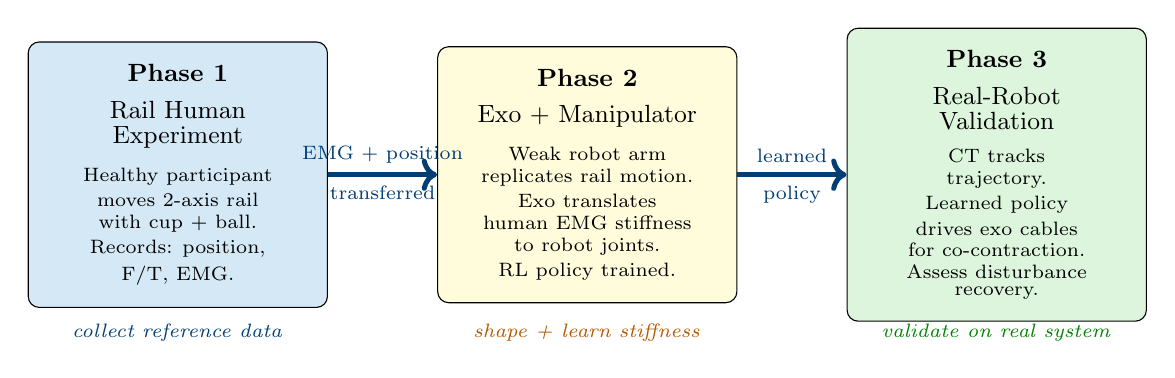
\begin{tikzpicture}[x=1cm,y=1cm,
  phase/.style={draw, rounded corners=4pt, minimum width=3.8cm, minimum height=2.6cm,
                align=center, font=\small, inner sep=8pt},
  label/.style={font=\small\bfseries, align=center},
  sub/.style={font=\scriptsize, align=center},
  arr/.style={->, very thick, color=imperialblue, line width=1.8pt}]

  %% Phase 1
  \node[phase, fill=lightblue] (p1) at (0,0)
    {\shortstack{\textbf{Phase 1}\\[4pt]Rail Human\\Experiment\\[4pt]
    \scriptsize Healthy participant\\
    \scriptsize moves 2-axis rail\\
    \scriptsize with cup + ball.\\
    \scriptsize Records: position,\\
    \scriptsize F/T, EMG.}};

  %% Phase 2
  \node[phase, fill=lightyellow] (p2) at (5.2,0)
    {\shortstack{\textbf{Phase 2}\\[4pt]Exo + Manipulator\\[4pt]
    \scriptsize Weak robot arm\\
    \scriptsize replicates rail motion.\\
    \scriptsize Exo translates\\
    \scriptsize human EMG stiffness\\
    \scriptsize to robot joints.\\
    \scriptsize RL policy trained.}};

  %% Phase 3
  \node[phase, fill=lightgreen] (p3) at (10.4,0)
    {\shortstack{\textbf{Phase 3}\\[4pt]Real-Robot\\Validation\\[4pt]
    \scriptsize CT tracks\\
    \scriptsize trajectory.\\
    \scriptsize Learned policy\\
    \scriptsize drives exo cables\\
    \scriptsize for co-contraction.\\
    \scriptsize Assess disturbance\\
    \scriptsize recovery.}};

  %% Arrows
  \draw[arr] (p1.east) -- node[above, font=\scriptsize]{EMG + position} node[below,font=\scriptsize]{transferred} (p2.west);
  \draw[arr] (p2.east) -- node[above, font=\scriptsize]{learned} node[below,font=\scriptsize]{policy} (p3.west);

  %% Phase labels below
  \node[sub, text=imperialblue] at (0,-2.0)  {\textit{collect reference data}};
  \node[sub, text=orange!70!black] at (5.2,-2.0) {\textit{shape + learn stiffness}};
  \node[sub, text=green!50!black] at (10.4,-2.0) {\textit{validate on real system}};
\end{tikzpicture}
\caption{Three-phase experimental sequence. Phase~1 records healthy human behaviour on the rail. Phase~2 builds a digital twin of the manipulator--exosuit and trains an RL policy that reproduces the desired Cartesian impedance. Phase~3 deploys the learned policy on the real robot: the CT controller handles trajectory tracking and the learned policy drives the exo cables to produce co-contraction and stiffness modulation.}
\label{fig:three-phase}
\end{figure}

\bigskip
This section formalises the three-step technical pipeline that connects
the human rail experiment to the simulated exosuit manipulator.

% -------------------------------------------------------------------------
\subsection{Phase-Wise Protocol and Data Mapping}
\label{sec:phasewise-transfer}
% -------------------------------------------------------------------------

\subsubsection{Phase 1 --- Human Rail Experiment (Master Side)}
\textbf{Objective.} Collect high-quality reference behaviour from healthy participants while they perform the rail cup-and-ball task.

\textbf{Operational steps.}
\begin{enumerate}[nosep]
  \item Run Block A (familiarisation, no ball) to learn rail dynamics and timing.
  \item Run Block B (ball-in-cup tracking) to capture nominal stabilisation behaviour.
  \item Run Block C (disturbance adaptation) to capture corrective and recovery behaviour.
  \item Record all streams with a common timestamp: rail position, F/T, EMG, camera-based ball state, disturbance trigger.
  \item Perform quality checks per trial (signal dropout, clipping, tracking loss, sync quality).
\end{enumerate}

\textbf{Block definitions inside Phase 1.}

\paragraph{Block A: Familiarisation without the ball.}
In Block A, participants complete 10 trials without the ball. The aim is to let
them learn the platform dynamics and become familiar with how hand motion affects
the two-rail system.

Participants are asked to move the platform left to right, right to left, and
up and down within a specified time window. Feedback is auditory: a pleasant
sound for successful completion and an unpleasant sound for failure.

\begin{figure}[H]
\centering
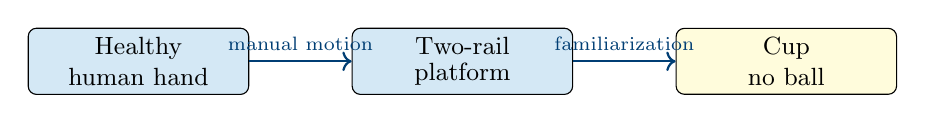
\begin{tikzpicture}[node distance=0.9cm and 1.3cm,
  box/.style={draw, rounded corners=3pt, minimum width=2.8cm, minimum height=0.8cm, fill=lightblue, align=center, font=\small},
  arr/.style={->, thick, color=imperialblue}]
  \node[box] (human) {\shortstack{Healthy\\human hand}};
  \node[box, right=of human] (rail) {\shortstack{Two-rail\\platform}};
  \node[box, right=of rail, fill=lightyellow] (cup) {\shortstack{Cup\\no ball}};
  \draw[arr] (human) -- node[above,font=\scriptsize]{manual motion} (rail);
  \draw[arr] (rail) -- node[above,font=\scriptsize]{familiarization} (cup);
\end{tikzpicture}
\caption{Phase-1 Block A schematic. Participants learn the rail motion without the ball so the platform dynamics can be learned first.}
\label{fig:block-a}
\end{figure}

\paragraph{Block B: Ball-in-cup control task.}
In Block B, the ball is added to the cup. A circular target region is defined,
and participants move the platform while keeping the ball inside the target as
much as possible.

Success can be defined by one or more criteria: completion within the time
limit, ball remaining inside the target circle, and boundary violations below
a threshold.

\begin{figure}[H]
\centering
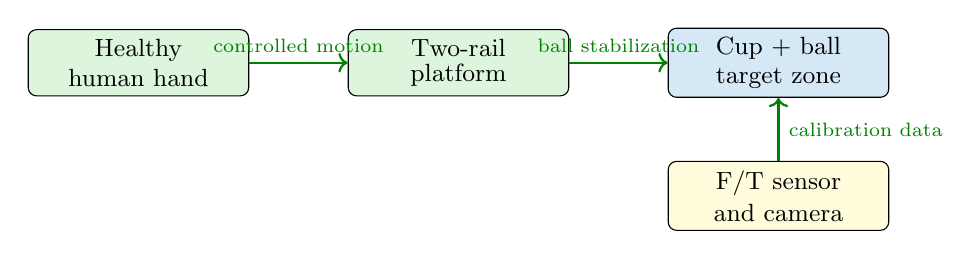
\begin{tikzpicture}[node distance=0.8cm and 1.25cm,
  box/.style={draw, rounded corners=3pt, minimum width=2.8cm, minimum height=0.8cm, fill=lightgreen, align=center, font=\small},
  arr/.style={->, thick, color=green!50!black}]
  \node[box] (human) {\shortstack{Healthy\\human hand}};
  \node[box, right=of human] (rail) {\shortstack{Two-rail\\platform}};
  \node[box, right=of rail, fill=lightblue] (cup) {\shortstack{Cup + ball\\target zone}};
  \node[box, below=0.8cm of cup, fill=lightyellow] (sense) {\shortstack{F/T sensor\\and camera}};
  \draw[arr] (human) -- node[above,font=\scriptsize]{controlled motion} (rail);
  \draw[arr] (rail) -- node[above,font=\scriptsize]{ball stabilization} (cup);
  \draw[arr] (sense) -- node[right,font=\scriptsize]{calibration data} (cup);
\end{tikzpicture}
\caption{Phase-1 Block B schematic. The ball must stay near the target while the participant moves the rail platform.}
\label{fig:block-b}
\end{figure}

\paragraph{Block C: Disturbance adaptation.}
In Block C, an external disturbance is introduced using a solenoid actuator
that pushes the rail toward the participant. The perturbation disturbs platform
motion and moves the ball away from the desired region.

Participants adapt their control strategy over repeated trials to bring the ball
back to target. This block probes disturbance rejection, error-based motor
learning, and recovery dynamics.

\begin{figure}[H]
\centering
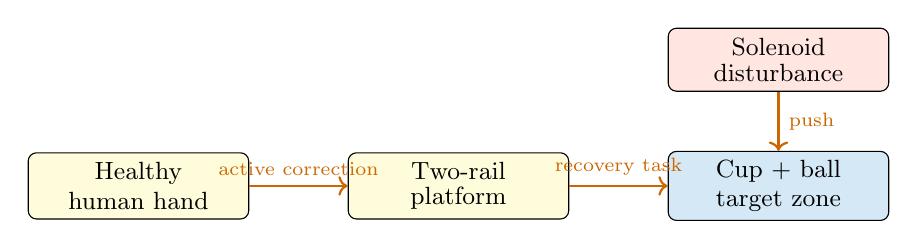
\begin{tikzpicture}[node distance=0.8cm and 1.25cm,
  box/.style={draw, rounded corners=3pt, minimum width=2.8cm, minimum height=0.8cm, fill=lightyellow, align=center, font=\small},
  arr/.style={->, thick, color=orange!80!black}]
  \node[box] (human) {\shortstack{Healthy\\human hand}};
  \node[box, right=of human] (rail) {\shortstack{Two-rail\\platform}};
  \node[box, right=of rail, fill=lightblue] (cup) {\shortstack{Cup + ball\\target zone}};
  \node[box, above=0.75cm of cup, fill=lightred] (dist) {\shortstack{Solenoid\\disturbance}};
  \draw[arr] (human) -- node[above,font=\scriptsize]{active correction} (rail);
  \draw[arr] (rail) -- node[above,font=\scriptsize]{recovery task} (cup);
  \draw[arr] (dist) -- node[right,font=\scriptsize]{push} (cup);
\end{tikzpicture}
\caption{Phase-1 Block C schematic. A disturbance pushes the rail, and the participant learns to recover the ball back to the target.}
\label{fig:block-c}
\end{figure}

\textbf{Rail setup diagrams for Phase 1.}
The physical and top-view rail geometries used in Phase 1 are shown in
Figs.~\ref{fig:rail-setup} and \ref{fig:rail-top-view}. These diagrams define
the coordinate axes, coaxial cup-handle mounting, and sensor placements used
for data collection and calibration.

\textbf{Data products from Phase 1.}
\begin{itemize}[nosep]
  \item Trajectory reference: $(x_c(t),y_c(t))$
  \item Interaction force reference: $\mathbf F(t)$
  \item Muscle activation/co-contraction features: $\mathbf P(t)$, $\mathbf P_{\text{null}}(t)$
  \item Ball-state performance labels: dwell time, boundary violations, recovery time
\end{itemize}

\subsubsection{Phase 2 --- Exo + Manipulator (Digital Twin and RL)}
\textbf{Objective.} Build a digital twin of the manipulator--exosuit system that captures robot dynamics, cable transmission, SEA compliance, and elbow stiffness modulation. Train an RL policy in the digital twin to reproduce the desired Cartesian impedance behaviour from the Phase~1 human demonstrations.

\textbf{Operational steps.}
\begin{enumerate}[nosep]
  \item Feed rail position $(x_c,y_c)$ into IK to generate joint references $\bq^*(t)$.
  \item Run weak-baseline CT tracking on the manipulator.
  \item Convert EMG co-contraction feature $\mathbf P_{\text{null}}$ to stiffness increment via $\hat{\boldsymbol\Psi}$ and map to exo command $c_{\text{exo}}$.
  \item Apply exo cable co-contraction in real time; this adds mechanical stiffness to the weak arm.
  \item Collect closed-loop robot rollout data and train policy (imitation pretraining + RL fine tuning).
\end{enumerate}

\textbf{Data products from Phase 2.}
\begin{itemize}[nosep]
  \item Robot state-action trajectories $(\bm s_t,\bm a_t)$
  \item Exo stiffness command trajectory $c_{\text{exo}}(t)$
  \item Task outcomes under assisted stiffness (ball error, tracking error, effort)
  \item Policy parameters $\pi_\theta$ and validation metrics
\end{itemize}

\subsubsection{Phase 3 --- Real-Robot Validation (Learned Policy via Exo)}
\textbf{Objective.} Deploy the trained RL policy on the physical manipulator--exosuit and validate whether exosuit-mediated stiffness shaping improves tracking stability and recovery under real-world disturbances.

\textbf{Operational steps.}
\begin{enumerate}[nosep]
  \item Connect the learned policy $\pi_\theta$ to the exo co-contraction command path, replacing the EMG-based Tele-Impedance signal from Phase~2.
  \item The CT controller continues to handle end-point trajectory tracking independently.
  \item The learned policy generates the antagonistic cable pre-tension setpoint $c_{\text{exo}}(t)$, physically producing co-contraction and stiffness modulation through the elbow exosuit.
  \item Run validation trials: nominal ball-in-cup tracking and disturbance recovery (same perturbation protocol as Phase~1 Block~C).
  \item Compare Exo OFF (CT only) against Exo ON (CT + learned policy) to quantify the benefit of exosuit-mediated stiffness shaping.
\end{enumerate}

\textbf{Success criteria.}
\begin{itemize}[nosep]
  \item Ball stabilisation metrics under the learned policy match or exceed Phase~2 (EMG-driven) performance.
  \item Disturbance recovery is faster and more repeatable with the learned policy driving the exo than without.
  \item The co-contraction profile is interpretable: stiffness increases near perturbations.
  \item Cable tensions and control effort remain within safe operational limits.
\end{itemize}

\subsubsection{Cross-Phase Data-to-Use Mapping}
\begin{center}
{\small
\begin{tabular}{p{0.28\linewidth}p{0.30\linewidth}p{0.34\linewidth}}
\toprule
\textbf{Signal (Phase 1)} & \textbf{Used in Phase 2} & \textbf{Used in Phase 3} \\
\midrule
Rail position $(x_c,y_c)$ & IK reference for $\bq^*(t)$ & Same task reference for final validation \\
EMG envelope $\mathbf P$ & Co-contraction extraction and exo command & Policy feature or distilled gain schedule input \\
F/T at handle & Calibration of $\hat{\mathbf T}$ and stiffness identification & Benchmark for interaction similarity \\
Ball state (camera/F/T map) & RL reward and trial scoring & Final autonomous performance scoring \\
Disturbance timing/amplitude & Robustness training episodes & Robustness validation episodes \\
\bottomrule
\end{tabular}}
\end{center}

% -------------------------------------------------------------------------
\subsection{Step 1 --- Coordinate Mapping: Rail Cart to Manipulator End-Effector}
% -------------------------------------------------------------------------

The two-rail platform defines a 2-D Cartesian position
$\bm{p}_{\text{rail}}(t) = [x_c(t),\, y_c(t)]^\top \in \mathbb{R}^2$,
measured by the rail encoders or Optitrack.  The manipulator
end-effector (cup tip) must follow the same trajectory in the workspace.

\paragraph{Forward kinematics (FK).}
Let $\bq = [q_1, q_2]^\top$ be the shoulder and elbow joint angles of
the 2-DOF cable-driven manipulator (link lengths $L_1$, $L_2$).
The cup tip position in the world frame is

\begin{align}
  p_x &= L_1 \cos q_1 + L_2 \cos(q_1 + q_2), \\
  p_y &= L_1 \sin q_1 + L_2 \sin(q_1 + q_2).
\end{align}

\paragraph{Inverse kinematics (IK).}
Given $\bm{p}_{\text{ref}}(t) = \bm{p}_{\text{rail}}(t)$ the required
joint trajectory is obtained by solving

\[
  \bq^*(t) = \arg\min_{\bq} \|\bm{p}(\bq) - \bm{p}_{\text{ref}}(t)\|^2,
\]

subject to joint limits.  In the simulation this is solved numerically at
each trajectory sample using Drake's \texttt{InverseKinematics} class
with warm-starting (previous solution used as seed).  The rail workspace
is chosen so that the two-link arm can cover the full travel without
reaching a singular configuration.

\paragraph{Practical workflow in simulation.}
\begin{enumerate}[nosep]
  \item Rail encoder/Optitrack streams
        $\bm{p}_{\text{rail}}(t)$ at the control rate ($\sim$200\,Hz).
  \item IK solves for $\bq^*(t)$; the result is the position setpoint.
  \item The computed-torque controller
        (\texttt{controller/computed\_torque\_isaacsim.py}) tracks
        $\bq^*(t)$ on the simulated manipulator.
  \item The SEA exo cables simultaneously receive the co-contraction
        setpoint derived from EMG (Section~\ref{sec:teleimpedance-method}).
\end{enumerate}

\begin{warnbox}
  \textbf{Joint-order note (Drake).}  Drake returns joint indices in URDF
  parse order, not alphabetical.  For \texttt{cup\_manipulator.urdf} the
  ordering is \texttt{[link2\_link1, link1\_base]}, i.e.\ the state vector is
  $[q_2, q_1]^\top$.  Always verify with \texttt{plant.GetJointIndices()} before
  setting IK seeds or reading solutions.
\end{warnbox}

% -------------------------------------------------------------------------
\subsection{Step 2 --- Weak-Stiffness Manipulator Model}
% -------------------------------------------------------------------------

The manipulator is intentionally operated with \emph{reduced} joint
stiffness to emulate an impaired or unhealthy limb.  In the computed-torque
(CT) framework the desired joint torque is

\begin{equation}
  \btau = \bM(\bq)\ddot{\bq}^* + \bC(\bq,\dot{\bq})\dot{\bq}
        + \bG(\bq)
        + K_p^{\text{eff}}\,(\bq^*-\bq)
        + K_d^{\text{eff}}\,(\dot{\bq}^*-\dot{\bq}),
\end{equation}

where the \emph{effective} PD gains are split into a weak baseline and an
exo-augmented increment:

\begin{align}
  K_p^{\text{eff}} &= K_p^{\text{weak}} + \Delta K_p^{\text{exo}}, \\
  K_d^{\text{eff}} &= K_d^{\text{weak}} + \Delta K_d^{\text{exo}}.
\end{align}

The weak-baseline gains satisfy $K_p^{\text{weak}} = \varepsilon\,
K_p^{\text{healthy}}$ with $\varepsilon \ll 1$ (typical range
$\varepsilon \in [0.1, 0.3]$), and the exo increment
$\Delta K_p^{\text{exo}} \geq 0$ is contributed by the exo-cable
co-contraction (dual-groove elbow pulley, Method~A/B).

At the SEA level the exo cable pretension $T_c$ adds to the joint
stiffness as

\begin{equation}
  \Delta K_p^{\text{exo}} \approx \frac{r_p^2\,k_s}{1}\,c_{\text{exo}},
\end{equation}

where $r_p$ is the pulley radius, $k_s$ is the SEA spring stiffness, and
$c_{\text{exo}} \in [0,1]$ is the dimensionless co-contraction command.
This relation is the link between the Tele-Impedance stiffness increment
$\Delta\mathbf{K}$ (identified in Stage-2 calibration) and the physical
cable setpoint.

\begin{center}
{\small
\begin{tabular}{llll}
\toprule
\textbf{Mode} & $K_p^{\text{weak}}$ & $\Delta K_p^{\text{exo}}$ & \textbf{Description} \\
\midrule
Healthy baseline & $K_p^{\text{healthy}}$ & 0 & full CT, no exo \\
Weak (impaired)  & $\varepsilon K_p^{\text{healthy}}$ & 0 & emulates impaired control \\
Weak + exo OFF   & $\varepsilon K_p^{\text{healthy}}$ & 0 & rail EMG not yet connected \\
Weak + exo ON    & $\varepsilon K_p^{\text{healthy}}$ & $\Delta K_p^{\text{exo}}(t)$ & live EMG-driven co-contraction \\
Learned          & $K_p^{\text{learned}}(t)$ & 0 & exo distilled into CT gains \\
\bottomrule
\end{tabular}}
\end{center}

% -------------------------------------------------------------------------
\subsection{Step 3 --- Exo-Informed Stiffness Learning}
% -------------------------------------------------------------------------

The long-term goal is for the manipulator to \emph{inherit} the stiffness
modulation that the exo currently provides, so the exo can eventually be
removed and the manipulator controller reproduces the same interaction
behavior autonomously.

\paragraph{Learning formulation.}
Define the state $\bm{s}(t) = [\bq, \dot{\bq},
\bm{p}_{\text{ball}}, \dot{\bm{p}}_{\text{ball}}, \bm{p}_{\text{rail}}]$
and the action $\bm{a}(t) = [c_{\text{exo}}, \btau_{\text{ff}}]$ (exo
co-contraction setpoint plus optional feed-forward torque adjustment).  The
RL policy

\[
  \bm{a}(t) = \pi_\theta(\bm{s}(t))
\]

is trained to minimise a cost function that rewards ball retention and
smooth rail tracking:

\begin{equation}
  \mathcal{J} = \mathbb{E}\!\left[\int_0^T
    \underbrace{w_1 \|\bm{p}_{\text{ball}} - \bm{p}_{\text{target}}\|^2}_{
        \text{ball position error}}
    + \underbrace{w_2 \|\bm{p}_{\text{EE}} - \bm{p}_{\text{rail}}\|^2}_{
        \text{EE tracking error}}
    + \underbrace{w_3 \|\btau\|^2}_{
        \text{effort penalty}}
    + \underbrace{w_4 \|\mathbf{K}_{\text{eff}}(t) - \mathbf{K}_{\text{ref}}(t)\|_F^2}_{
        \text{impedance matching}}
    \,\mathrm{d}t\right],
\end{equation}

The fourth term rewards matching the Cartesian stiffness reference
$\mathbf{K}_{\text{ref}}(t)$ estimated from Phase~1 human EMG and posture
data, which encourages the policy to produce co-contraction that mirrors the
human impedance response---in particular increasing $c_{\text{exo}}$ near
perturbations.

Data collected during \emph{Weak + exo ON} trials (where the exo acts as a
teacher) provide the demonstration set for imitation-learning pre-training;
PPO fine-tunes the policy thereafter.

\paragraph{Policy deployment through the exosuit (Phase 3).}
Once $\pi_\theta$ is trained in the digital twin, it is deployed on the real
manipulator--exosuit with the exo hardware still present. The EMG-based
Tele-Impedance co-contraction command is replaced by the policy output:

\begin{equation}
  c_{\text{exo}}(t) = \pi_\theta^{(c)}(\bm{s}(t)),
\end{equation}

where $\pi_\theta^{(c)}$ is the co-contraction output channel of the trained
policy and $\bm{s}(t)$ contains robot joint states, end-effector motion, and
interaction information.  The CT controller continues to track the end-point
trajectory independently.  This two-channel architecture (position via CT,
stiffness via learned exo policy) mirrors the Tele-Impedance master--slave
structure of Section~\ref{sec:teleimpedance-method} but replaces the human
operator's EMG with an autonomous policy.  Experimental evaluation then
assesses whether exosuit-mediated stiffness shaping improves tracking
stability and disturbance recovery relative to the no-exo (CT-only) baseline.

\begin{figure}[H]
\centering
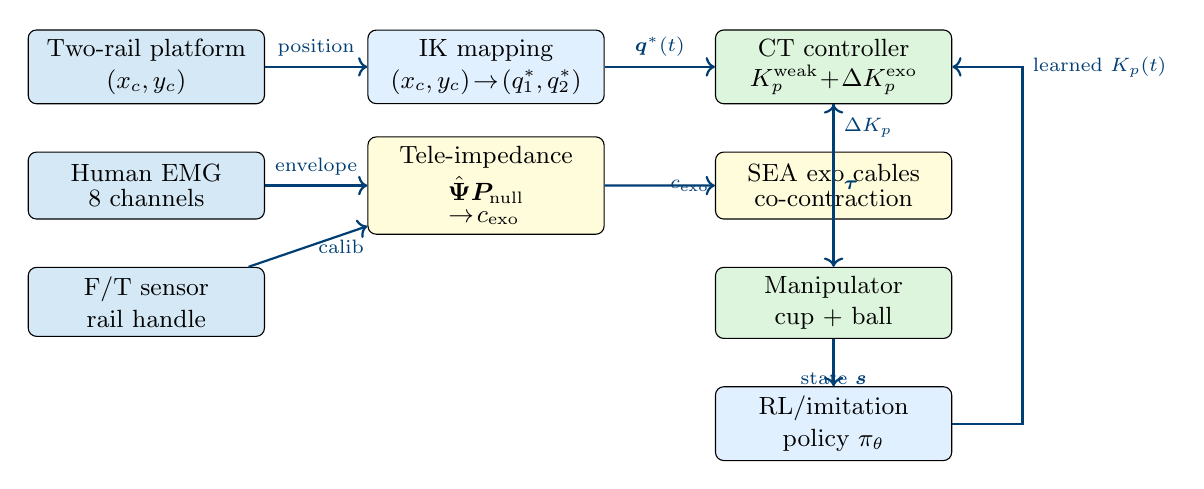
\begin{tikzpicture}[node distance=0.65cm and 1.1cm,
  box/.style={draw, rounded corners=3pt, minimum width=3.0cm, minimum height=0.85cm,
              align=center, font=\small},
  hbox/.style={box, fill=lightblue},
  rbox/.style={box, fill=lightgreen},
  ebox/.style={box, fill=lightyellow},
  lbox/.style={box, fill=actionblue},
  arr/.style={->, thick, color=imperialblue}]

  %% Human (master) side
  \node[hbox] (rail)  {\shortstack{Two-rail platform\\$(x_c,y_c)$}};
  \node[hbox, below=0.6cm of rail] (emg) {\shortstack{Human EMG\\8 channels}};
  \node[hbox, below=0.6cm of emg]  (ft)  {\shortstack{F/T sensor\\rail handle}};

  %% IK block
  \node[lbox, right=1.3cm of rail]  (ik)  {\shortstack{IK mapping\\$(x_c,y_c)\!\to\!(q_1^*,q_2^*)$}};

  %% Stiffness estimation
  \node[ebox, right=1.3cm of emg]   (tci) {\shortstack{Tele-impedance\\$\hat{\boldsymbol\Psi}\bm{P}_\text{null}$\\$\!\to\!c_\text{exo}$}};

  %% Manipulator (slave) side
  \node[rbox, right=1.4cm of ik]    (ct)  {\shortstack{CT controller\\$K_p^\text{weak}\!+\!\Delta K_p^\text{exo}$}};
  \node[ebox, below=0.6cm of ct]    (exo) {\shortstack{SEA exo cables\\co-contraction}};
  \node[rbox, below=0.6cm of exo]   (plant){\shortstack{Manipulator\\cup + ball}};

  %% RL policy
  \node[lbox, below=0.6cm of plant] (rl)  {\shortstack{RL/imitation\\policy $\pi_\theta$}};

  %% arrows
  \draw[arr] (rail) -- node[above,font=\scriptsize]{position} (ik);
  \draw[arr] (ik)   -- node[above,font=\scriptsize]{$\bq^*(t)$} (ct);
  \draw[arr] (emg)  -- node[above,font=\scriptsize]{envelope} (tci);
  \draw[arr] (tci)  -- node[right,font=\scriptsize]{$c_\text{exo}$} (exo);
  \draw[arr] (exo)  -- node[right,font=\scriptsize]{$\Delta K_p$} (ct);
  \draw[arr] (ct)   -- node[right,font=\scriptsize]{$\btau$} (plant);
  \draw[arr] (ft)   -- node[right,font=\scriptsize]{calib} (tci);
  \draw[arr] (plant) -- node[below,font=\scriptsize]{state $\bm{s}$} (rl);
  \draw[arr] (rl)   -- ++(2.4,0) |- node[right,font=\scriptsize]{learned $K_p(t)$} (ct);
\end{tikzpicture}
\caption{Full rail-to-manipulator transfer pipeline.  Left: human master side
(rail, EMG, F/T).  Right: robotic slave side (CT controller, SEA exo, manipulator
cup + ball).  The RL policy closes the loop by distilling exo-shaped stiffness
directly into the CT gain schedule, so the exo can eventually be removed.}
\label{fig:transfer-pipeline}
\end{figure}

\begin{infobox}
\textbf{Simulation entry points.}
\begin{itemize}[nosep]
  \item Exo co-contraction PyDrake simulation:
        \texttt{script\_cup\_manipulator\_pendulam\_tendon\_with\_exo\_pydrake.py}
  \item Isaac Sim version:
        \texttt{script\_cup\_manipulator\_pendulam\_tendon\_with\_exo\_isaac\_sim.py}
  \item CT controller (engine-agnostic):
        \texttt{controller/computed\_torque\_isaacsim.py}
  \item SEA cable model:
        \texttt{actuators/sea\_isaacsim.py}
  \item RL training:
        \texttt{rl/train\_ppo\_residual.py}
\end{itemize}
\end{infobox}

\bibliographystyle{plainnat}
\bibliography{refs_2026_05_26}

\end{document}
